
\subsection{The tracking system}
The tracking system of CMS \cite{Tracker_1, Tracker_2} is designed to provide a precise and efficient measurement of the trajectories of charged particles emerging from the LHC collisions, as well as a precise reconstruction of secondary vertices. It surrounds the interaction point and has a length of 5.8 m and a diameter of 2.5 m. The CMS solenoid provides a homogeneous magnetic field of 4 T over the full volume of the tracker. At the LHC design luminosity of $10^{34} cm^{-2} s^{-1}$ there will be on average about 1000 particles from more than 20 overlapping proton-proton interactions traversing the tracker for each bunch crossing, i.e. every 25 ns. Therefore a detector technology featuring high granularity and fast response is required, such that the trajectories can be identified reliably and attributed to the correct bunch crossing. \\
The CMS tracker is shown in \figurename~\ref{tracking_system}: it is composed of a pixel detector with three barrel layers at radii between 4.4 cm and 10.2 cm and a silicon strip tracker with 10 barrel detection layers extending outwards to a radius of 1.1 m. Each system is completed by endcaps which consist of 2 disks in the pixel detector and 3 plus 9 disks in the strip tracker on each side of the barrel, extending the acceptance of the tracker up to a pseudorapidity of $|\eta| < 2.5$.\\
\begin{figure}[htbp]
\centering
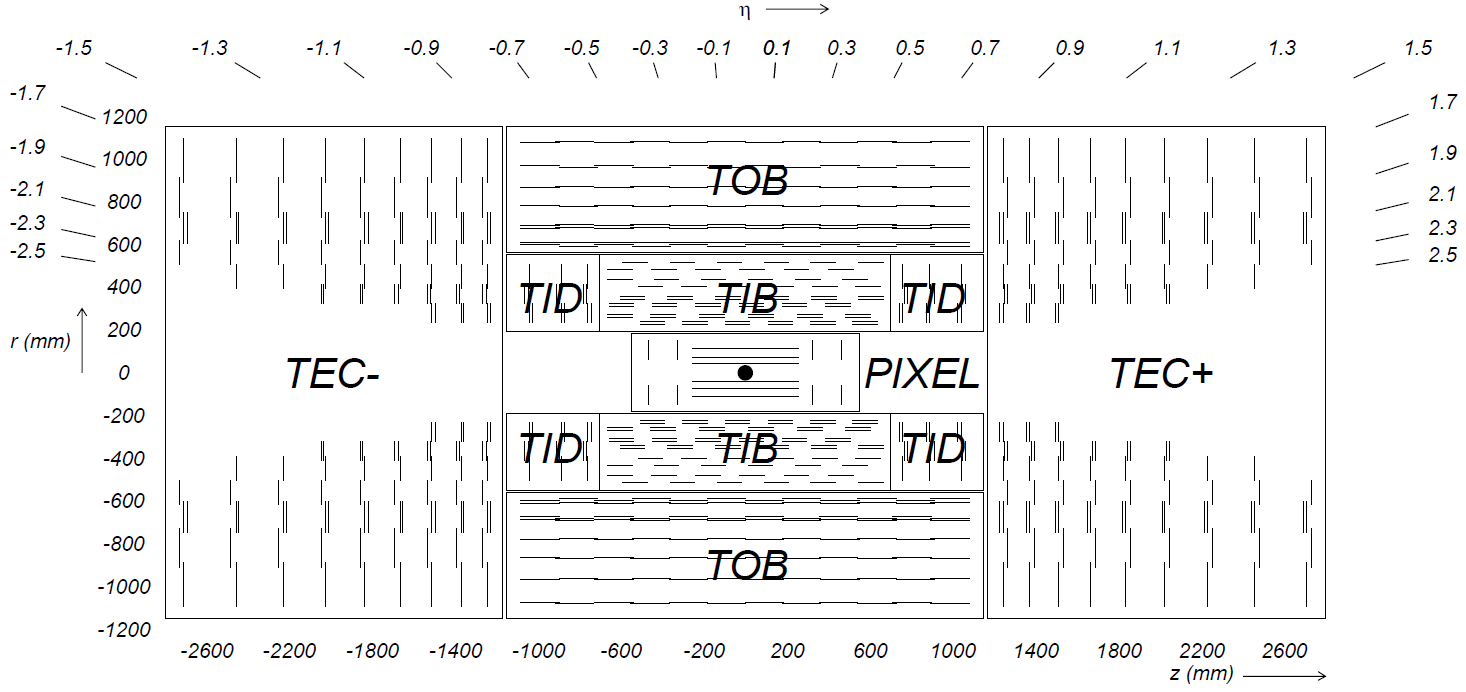
\includegraphics[width=0.7\textwidth]{Images/cmsTracker_TrackerLayout}
\caption{Schematic cross section through the CMS tracker in the $r-z$ plane: each line represents a detector module. Double lines indicate back-to-back modules which deliver stereo hits.}
\label{tracking_system}
\end{figure}
The tracker is the closest detector to the interaction point and it has a fundamental role in measuring kinematic variables of the particles. In \figurename~\ref{Tracker_performance} is shown the expected resolution of transverse momentum, transverse impact parameter and longitudinal impact parameter, as a function of pseudorapidity for single muons of transerve momentum of 1, 10 and 100 $GeV$. 
\begin{figure}[htbp]
\centering
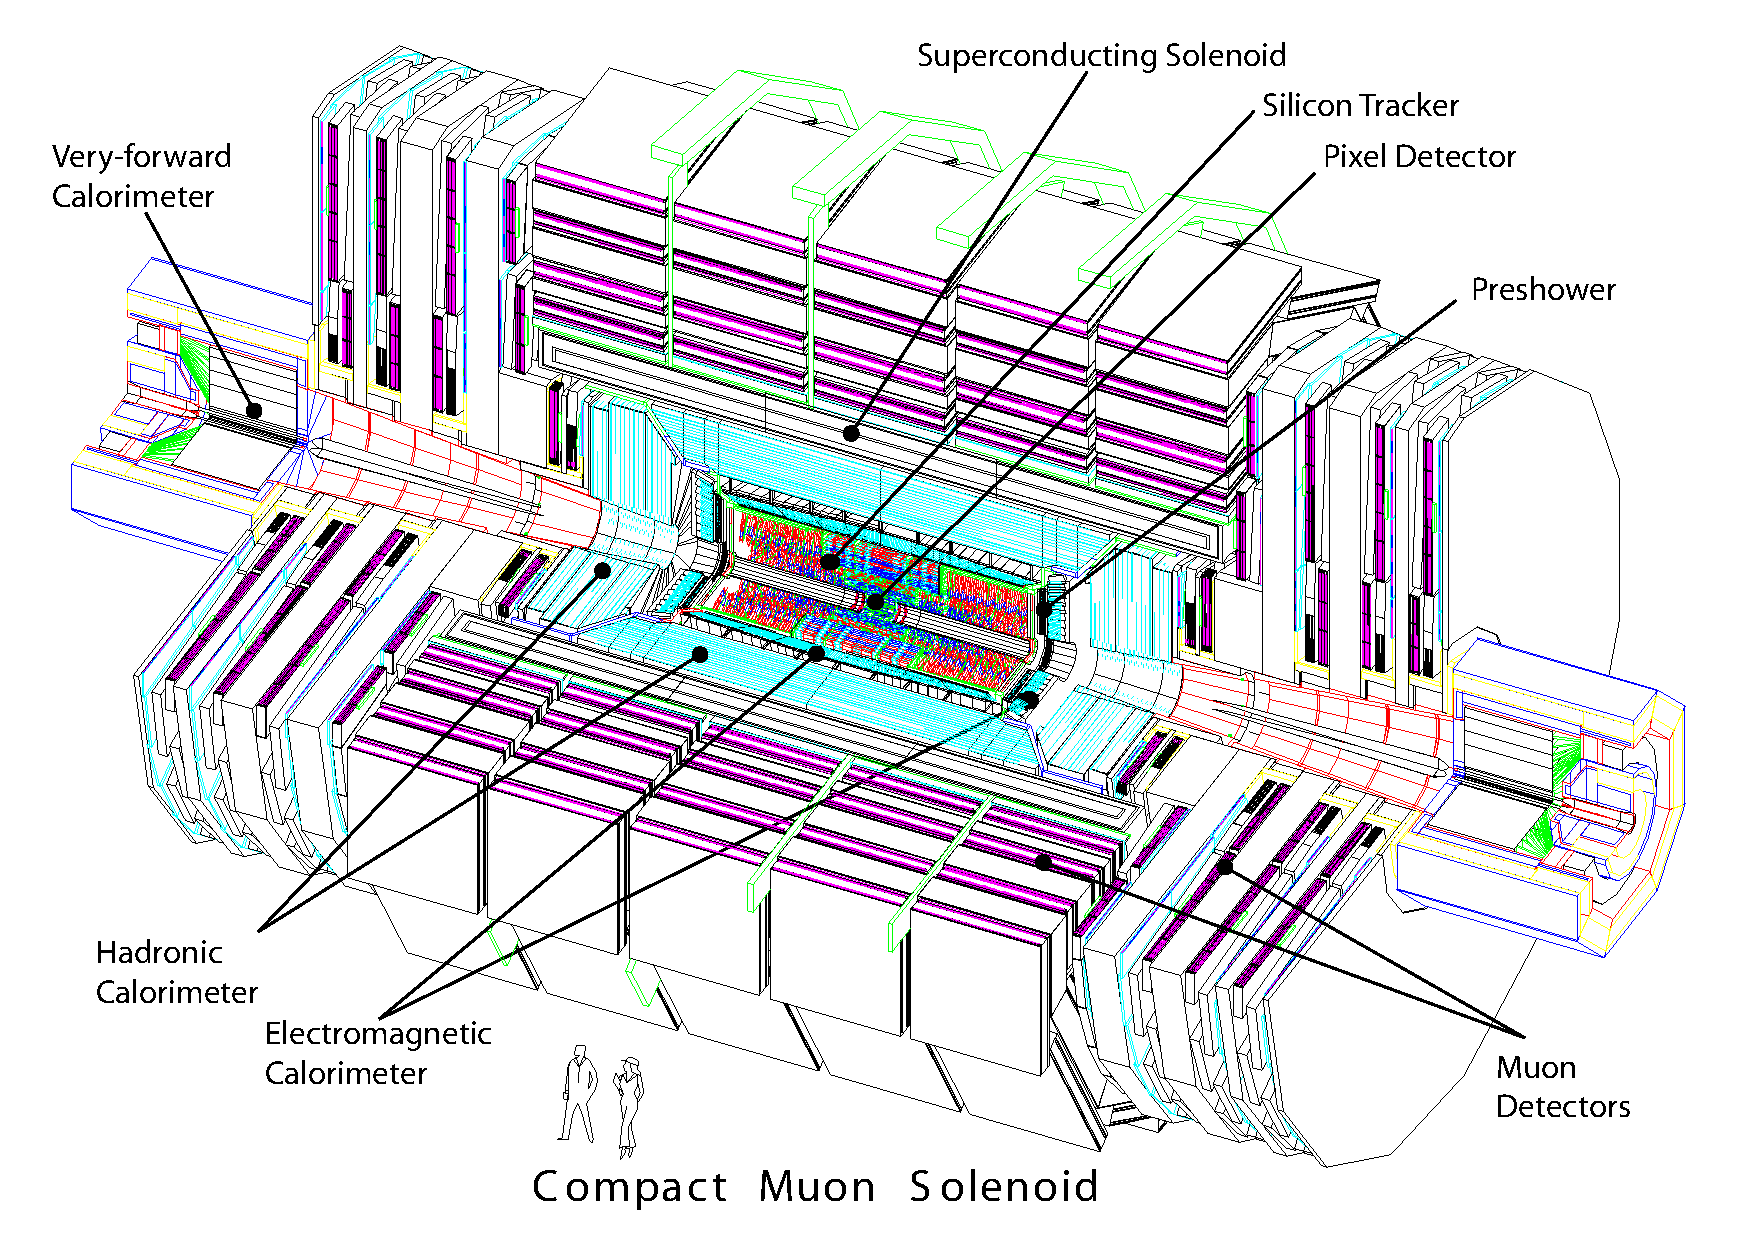
\includegraphics[width=0.1\textwidth]{Images/CMS_Layout.pdf}
\caption{Resolution for single muons with transverse momentum of 1, 10 and 100 GeV for several track parameters: transverse momentum (left panel), transverse impact parameter (middle panel), and longitudinal impact parameter (right panel).}
\label{Tracker_performance}
\end{figure}
For high momentum tracks (100 GeV) the transverse momentum resolution is around 1 - 2\% up to $|\eta| \approx 1.6$, beyond which it degrades due to the reduced lever arm. At a transverse momentum of 100 GeV multiple scattering in the tracker material accounts for 20 to 30\% of the transverse momentum resolution while at lower momentum it is dominated by multiple scattering. The transverse impact parameter resolution reaches 10 $\mu$m for high $p_{T}$ tracks, dominated by the resolution of the first pixel hit, while at lower momentum it is degraded by multiple scattering (similarly for the longitudinal impact parameter). \figurename~\ref{Tracker_performance}  shows the expected track reconstruction efficiency of the CMS tracker for single muons as a function of pseudorapidity: the efficiency is about 99\% over most of the acceptance and it decreases slightly at $|\eta| \approx 0$ due to gaps between the ladders of the pixel detector at z $\approx$ 0. At high $\eta$ the efficiency drop is mainly due to the reduced coverage by the pixel forward disks. \\ 
MATERIAL BUDGET
%Il tracker ricopre un?accettanza fino a |\eta| ? 2.5; `e spesso circa una lunghezza di radiazione e va da 0.4 X0 sulla verticale, crescendo fino a 1.8 X0 per |\eta| ? 1.4 e poi ridiscende ad una lunghezza per |\eta| ? 2.5.



\begin{figure}[htbp]
\centering
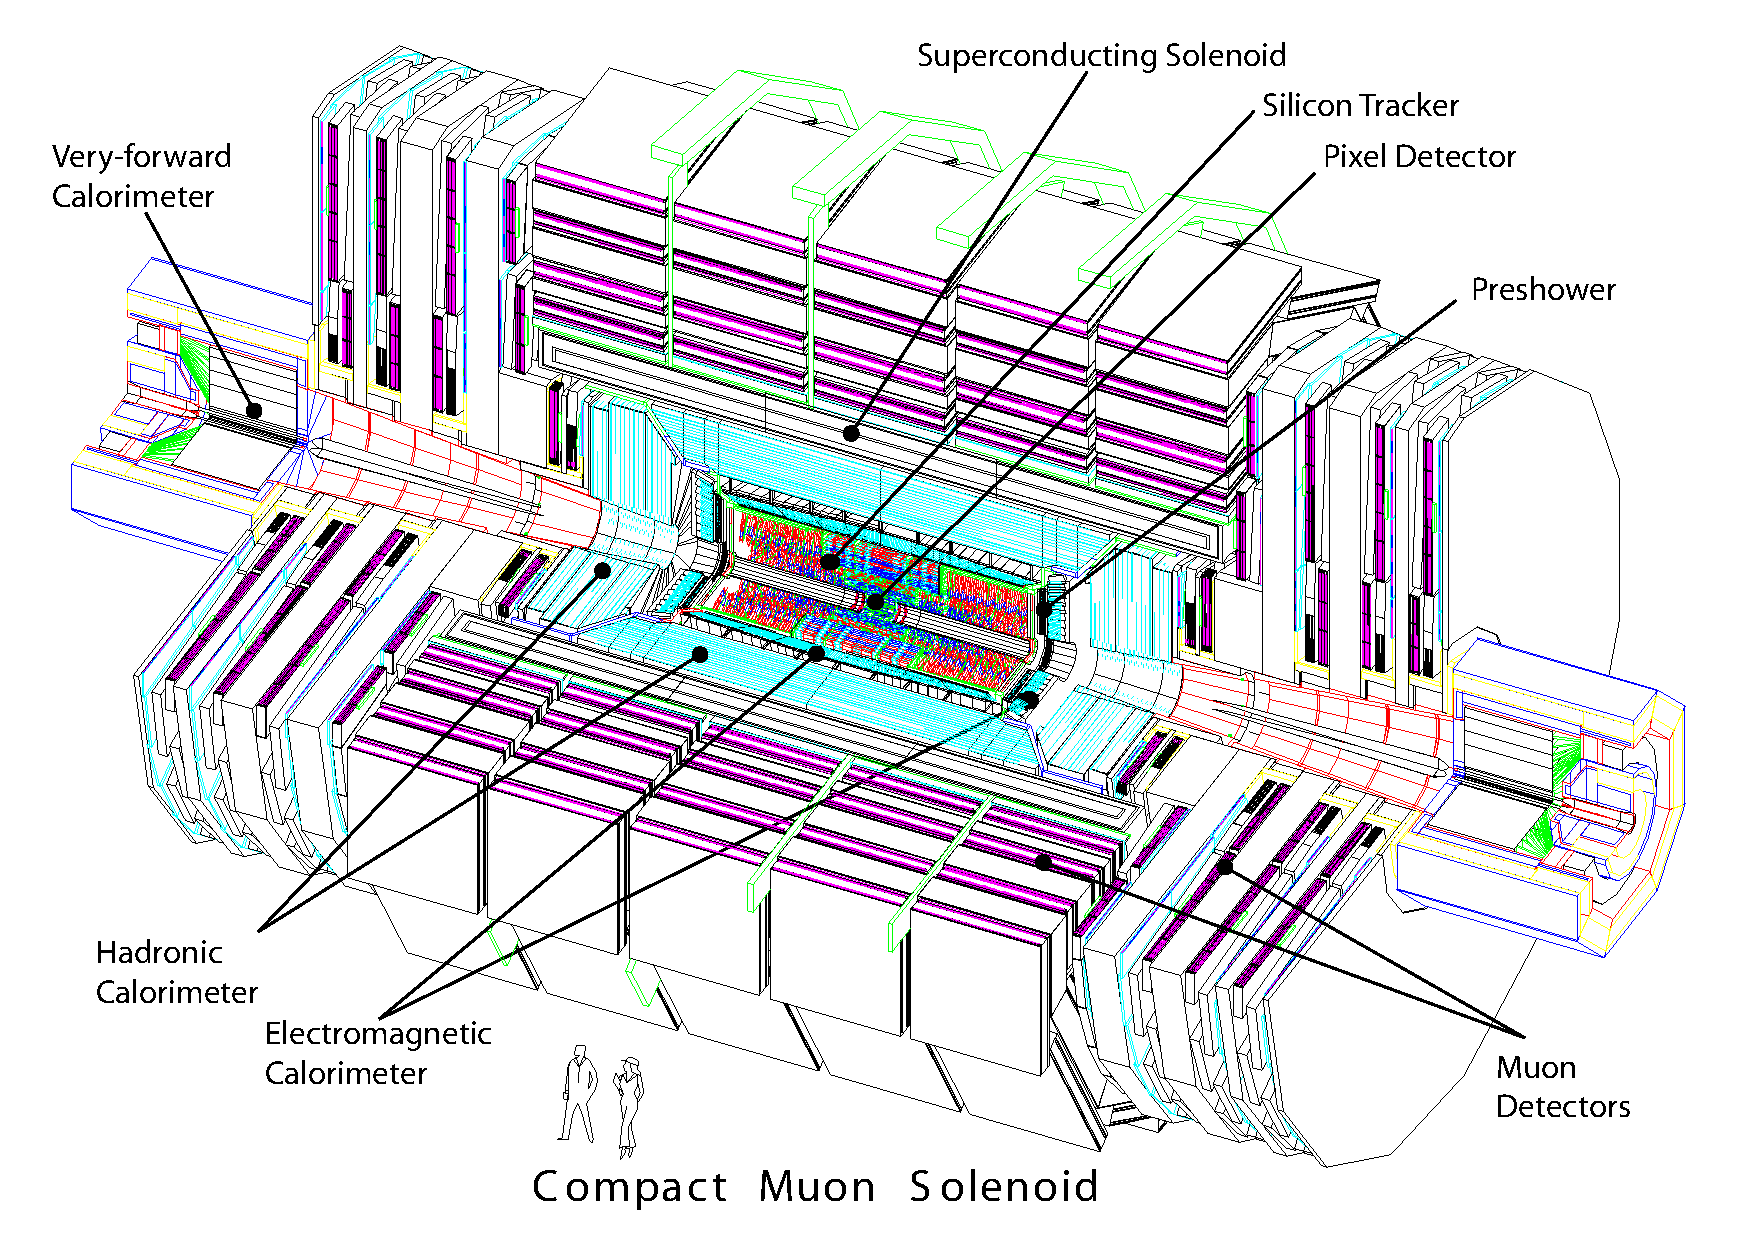
\includegraphics[width=0.1\textwidth]{Images/CMS_Layout.pdf}
\caption{Global track reconstruction efficiency for muons of several transverse momentum: 1, 10, 100 GeV.}
\label{Tracker_performance}
\end{figure}


\subsection{Electromagnetic calorimeter}
The electromagnetic calorimeter of CMS (ECAL) is a hermetic homogeneous calorimeter made of 61200 lead tungstate ($PbWO_{4}$) crystals mounted in the central barrel part, closed by 7324 crystals in each of the two endcaps. A preshower detector is placed in front of the endcap crystals. Avalanche photodiodes (APDs) are used as photodetectors in the barrel and vacuum phototriodes (VPTs) in the endcaps. The use of high density crystals has allowed the design of a calorimeter which is fast, has fine granularity and is radiation resistant. One of the driving criteria in the design was the capability to detect the decay to two photons of the postulated Higgs boson. \\
The characteristics \cite{PbWO4}  of the $PbWO_{4}$ crystals make them an appropriate choice for operation at LHC. The high density (8.28$g/cm^{3}$), short radiation length (0.89 cm) and small Moli�re radius (2.2 cm) result in a fine granularity and a compact calorimeter. The scintillation decay time of these crystals is of the same order of magnitude as the LHC bunch crossing time: about 80\% of the light is emitted in 25 ns. The light output is relatively low and varies with temperature: at 18$^\circ$C about 4.5 photoelectrons per MeV are collected in both APDs and VPTs. The crystals emit blue-green scintillation light with a broad maximum at 420?430 nm. \\
The barrel part of the ECAL (EB) covers the pseudorapidity range $|\eta|$ < 1.479. The barrel granularity is 360 fold in $\phi$ and (2x85) fold in $\eta$, resulting in a total of 61200 crystals. The crystals have a tapered shape, slightly varying with position in $\eta$. They are mounted in a quasi-projective geometry to avoid cracks aligned with particle trajectories, so that their axes make a small angle ($3^\circ$) with respect to the vector from the nominal interaction vertex, in both the $\phi$ and $\eta$ projections. The crystal cross-section corresponds to approximately 0.0174x0.0174 in $\eta-\phi$ or 22x22 $mm^{2}$ at the front face of crystal, and 26x26 $mm^{2}$ at the rear face. The crystal length is 230 mm corresponding to 25.8 $X_{0}$ (where the symbol  $X_{0}$ stands for a \textit{radiation length}). The barrel crystal volume is 8.14 $m^{3}$ and the weight is 67.4 t. The endcaps (EE) cover the rapidity range 1.479 < $|\eta|$ < 3.0. The longitudinal distance between the interaction point and the endcap envelope is 315.4 cm, taking account of the estimated shift toward the interaction point by 1.6 cm when the 4-T magnetic field is switched on. The endcap consists of identically shaped crystals grouped in mechanical units of 5x5 crystals (supercrystals, or SCs) consisting of a carbon-fibre alveola structure. Each endcap is divided into 2 halves, or Dees. Each Dee holds 3662 crystals. These are contained in 138 standard SCs and 18 special partial supercrystals on the inner and outer circumference. The crystals and SCs are arranged in a rectangular x-y grid, with the crystals pointing at a focus 1300 mm beyond the interaction point, giving off-pointing angles ranging from 2 to 8 degrees. The crystals have a rear face cross section 30x30 $mm^{2}$, a front face cross section 28.62x28.62 $mm^{2}$ and a length of 220 mm (24.7 $X_{0}$). The endcaps crystal volume is 2.90 $m^{3}$ and the weight is 24.0 t. The layout of the calorimeter is shown in \figurename~\ref{ECAL}. \\
\begin{figure}[htbp]
\centering
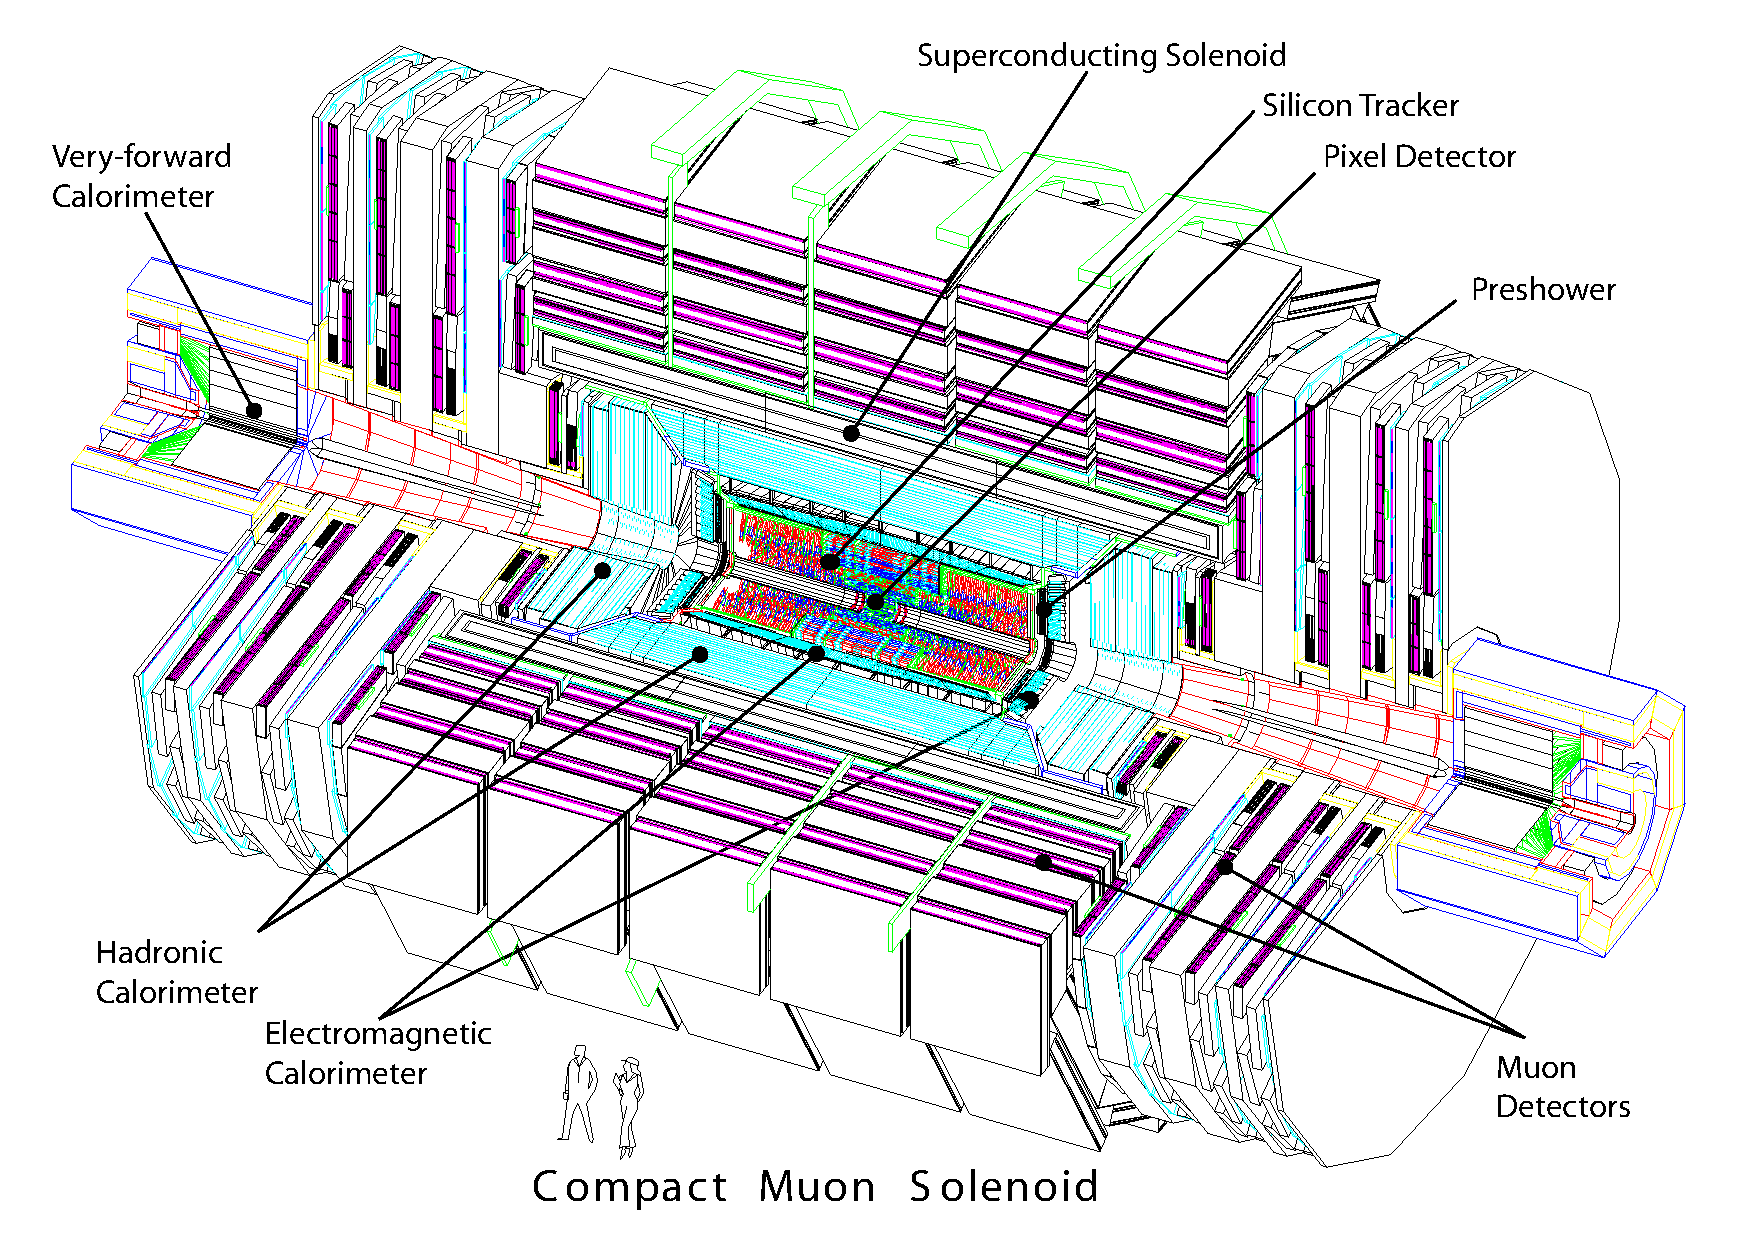
\includegraphics[width=0.1\textwidth]{Images/CMS_Layout.pdf}
\caption{Layout of the CMS electromagnetic calorimeter showing the arrangement of crystal modules, supermodules and endcaps, with the preshower in front.}
\label{ECAL}
\end{figure}

\subsubsection{Preshower detector}
The principal aim of the CMS Preshower detector is to identify neutral pions in the endcaps within a fiducial region 1.653 < $|\eta|$ < 2.6. It also helps the identification of electrons against minimum ionizing particles, and improves the position determination of electrons and photons with high granularity. The Preshower is a sampling calorimeter with two layers: lead radiators initiate electromagnetic showers from incoming photons/electrons whilst silicon strip sensors placed after each radia- tor measure the deposited energy and the transverse shower profiles. The total thickness of the Preshower is 20 cm. The material thickness of the Preshower traversed at $\eta$ = 1.653 before reaching the first sensor plane is 2 $X_{0}$, followed by a further 1 $X_{0}$ before reaching the second plane. Thus about 95\% of single incident photons start showering before the second sensor plane. The orientation of the strips in the two planes is orthogonal. 

\subsubsection{Energy resolution}
For energies below about 500 GeV, where shower leakage from the rear of the calorimeter starts to become significant, the energy resolution can be parametrized a:
\begin{equation}
\left(\frac{\sigma}{E}\right)^{2} = \left(\frac{S}{\sqrt{E}}\right)^2 + \left(\frac{N}{E}\right)^2  +C^{2}
\label{ECAL_resolution}
\end{equation}
where S is the stochastic term, N the noise term, and C the constant term. \\
The stochastic term has three basic contributions:
\begin{enumerate}
\item event-to-event fluctuations in the lateral shower containmen
\item a photostatistics contribution of 2.1\%
\item fluctuations in the energy deposited in the preshower absorber (where present) with respect to what is measured in the preshower silicon detector
\end{enumerate}
The contribution to the energy resolution from the preshower device can be approximately parametrized as a stochastic term with a value of 5\%/$\sqrt{E}$, where E is in GeV. But, because it samples only the beginning of the shower, the resolution is, in fact, predicted to vary like $\sigma$/E $\propto$ 1/$E^{0.75}$. \\
For the constant term instead, the main contributions are:
\begin{enumerate}
\item non-uniformity of the longitudinal light collection
\item intercalibration errors
\item leakage of energy from the back of the crystal
\end{enumerate}









